\newpage
\hypertarget{subSec:setupParser}{}
\subsection{Setting up the Parser}
\genHeader

\begin{itemize}

\item[$\blacktriangleright$] You working set generator node should now resemble Fig.~\ref{eclipse:generatedAdapter}. Be sure to take a look at the
\texttt{Moflon} and \texttt{Moca} library nodes that reference jars for all required dependencies.

\begin{figure}[htpb]
\begin{center}
  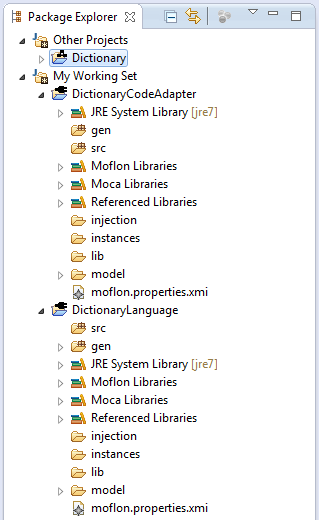
\includegraphics[width=0.4\textwidth]{eclipse_generatedAdapter}
  \caption{figureCaption}
  \label{eclipse:generatedAdapter}
\end{center}
\end{figure}

\item[$\blacktriangleright$] Right-click on \texttt{DictionaryCodeAdapter} and navigate to ``eMolfon/ Add Parser/Unparser'' (Fig~\ref{eclipse:contextParser}).

\begin{figure}[htpb]
\begin{center}
  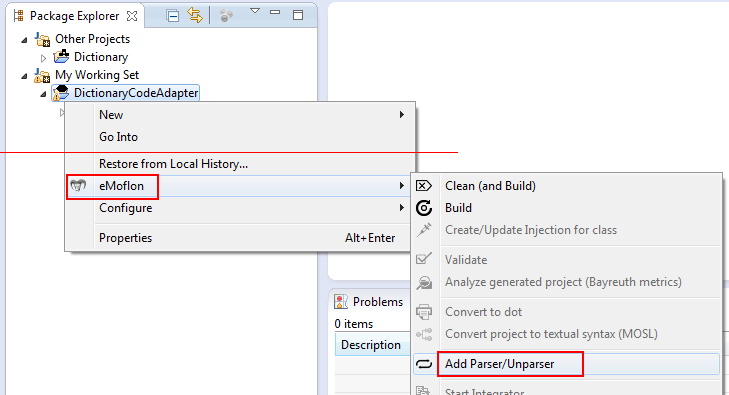
\includegraphics[width=0.9\textwidth]{eclipse_contextAddParserUnparser}
  \caption{figureCaption}
  \label{eclipse:contextParser}
\end{center}
\end{figure}

\item[$\blacktriangleright$] In the wizard dialogue (Fig~\ref{eclipse:wizardParser}), enter ``dictionary'' as the \texttt{File extension}, and make sure
the boxes \texttt{Create Parser} and \texttt{Create Unparser} with \texttt{ANTLR} are chosen as corresponding technology in both cases. Click \texttt{Finish} to
close.

\begin{figure}[htpb]
\begin{center}
  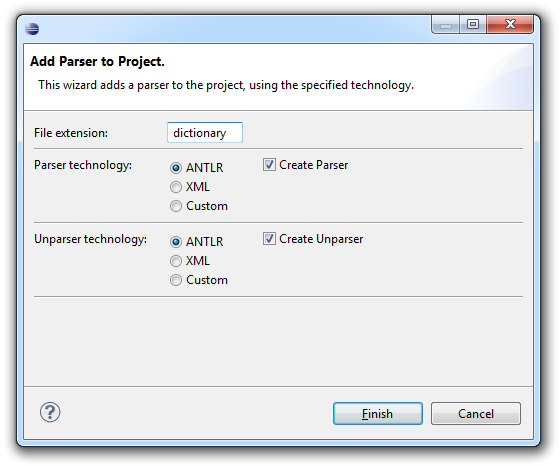
\includegraphics[width=0.8\textwidth]{eclipse_wizardParser}
  \caption{figureCaption}
  \label{eclipse:wizardParser}
\end{center}
\end{figure}

If everything has been installed and set up properly, parser and unparser stubs should be generated and \texttt{ANTLR} should automatically build the
corresponding Java code as depicted in Fig.~\ref{eclipse:generatedParser}.

\begin{figure}[htpb]
\begin{center}
  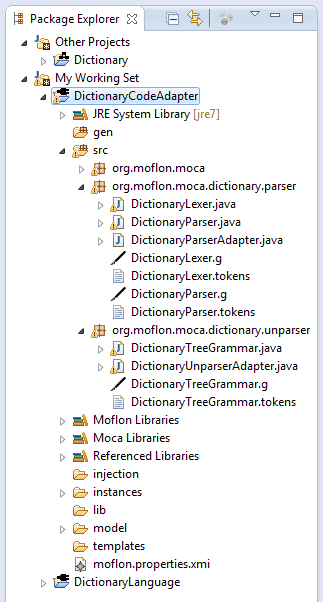
\includegraphics[width=0.4\textwidth]{eclipse_generatedParser}
  \caption{figureCaption}
  \label{eclipse:generatedParser}
\end{center}
\end{figure}

{\bf self:: update TGGMain and MocaMain so that tgg runs a round trip.}

\end{itemize}
